%niveau estimé : 4ème
    %date de projection : 18_11_2024
    %themes abordés : prix, ,
    
    \vspace{-0.5cm}
    \begin{multicols}{2}
        \boiteQFQ{Question 1 :}{
            Calculez le \textbf{nouveau prix} d'un article qui coûte $13{,}30$ \euro{} après une \textbf{réduction} de $5\%$ de son prix.
        }
        \boiteQFQ{Question 2 :}{
            \textbf{Déterminer} tous les \textbf{diviseurs} du nombre $\fpeval{3*5*7}$.
        }
    \end{multicols}
    \vspace{-0.85cm}
    \begin{multicols}{2}
        
        \boiteQFQ{Question 3 :}{
            \textbf{Calcule} la somme des fractions suivantes : \[\dfrac{5}{18} + \dfrac{5}{2}\]
        }
        \boiteQFA{}
    \end{multicols}
    
    \newpage
    \vspace{-0.5cm}
    \begin{multicols}{2}
        \boiteQFQ{Question 1 :}{
            Calculez le \textbf{nouveau prix} d'un article qui coûte $13{,}30$ \euro{} après une \textbf{réduction} de $5\%$ de son prix.
        }
        \boiteQFQ{Question 2 :}{
            \textbf{Déterminer} tous les \textbf{diviseurs} du nombre $\fpeval{3*5*7}$.
        }
        
    \end{multicols}
    \vspace{-0.85cm}
    \begin{multicols}{2}
        
        \boiteQFQ{Question 3 :}{
            \textbf{Calcule} la somme des fractions suivantes : \[\dfrac{5}{18} + \dfrac{5}{2}\]
        }
        \boiteQFA{
            \vspace{-0.35cm}
            \begin{itemize}[itemsep=0.2em]
                \item[\raisebox{-0.2cm}{\begin{itembox} \textbf{Q.1} \end{itembox}}] $ \num{12.64} ~$\euro{}
            \end{itemize}
        }
    \end{multicols}
    \newpage
    \vspace{-0.5cm}
    \begin{multicols}{2}
        \boiteQFQ{Question 1 :}{
            Calculez le \textbf{nouveau prix} d'un article qui coûte $13{,}30$ \euro{} après une \textbf{réduction} de $5\%$ de son prix.
        }
        \boiteQFQ{Question 2 :}{
            \textbf{Déterminer} tous les \textbf{diviseurs} du nombre $\fpeval{3*5*7}$.
        }
        
    \end{multicols}
    \vspace{-0.85cm}
    \begin{multicols}{2}
        
        \boiteQFQ{Question 3 :}{
            \textbf{Calcule} la somme des fractions suivantes : \[\dfrac{5}{18} + \dfrac{5}{2}\]
        }
        \boiteQFA{
            \vspace{-0.35cm}
            \begin{itemize}[itemsep=0.2em]
                \item[\raisebox{-0.2cm}{\begin{itembox} \textbf{Q.1} \end{itembox}}] $ \num{12.64} ~$\euro{}
                \item[\raisebox{-0.2cm}{\begin{itembox} \textbf{Q.2} \end{itembox}}] $1,3, 5, 7, 15,21,35,$ et \fpeval{3*5*7}
            \end{itemize}
        }
    \end{multicols}
    \newpage
    
    \begin{multicols}{2}
        \boiteQFQ{Question 1 :}{
            Calculez le \textbf{nouveau prix} d'un article qui coûte $13{,}30$ \euro{} après une \textbf{réduction} de $5\%$ de son prix.
        }
        \boiteQFQ{Question 2 :}{
            \textbf{Déterminer} tous les \textbf{diviseurs} du nombre $\fpeval{3*5*7}$.
        }
        
    \end{multicols}
    \vspace{-0.85cm}
    \begin{multicols}{2}
        
        \boiteQFQ{Question 3 :}{
            \textbf{Calcule} la somme des fractions suivantes : \[\dfrac{5}{18} + \dfrac{5}{2}\]
        }
        \boiteQFA{
            \vspace{-0.35cm}
            \begin{itemize}[itemsep=0.2em]
                \item[\raisebox{-0.2cm}{\begin{itembox} \textbf{Q.1} \end{itembox}}] $ \num{12.64} ~$\euro{}
                \item[\raisebox{-0.2cm}{\begin{itembox} \textbf{Q.2} \end{itembox}}] $1,3, 5, 7, 15,21,35,$ et \fpeval{3*5*7}
                \item[\raisebox{-0.2cm}{\begin{itembox} \textbf{Q.3} \end{itembox}}] $\dfrac{25}{9}$
            \end{itemize}
        }
    \end{multicols}
    
    \newpage
    
    %\begin{multicols}{2}
    \boiteQFdet{Question 1 :}{
        
        Calculez le \textbf{nouveau prix} d'un article qui coûte $13{,}30$ \euro{} après une \textbf{réduction} de $5\%$ de son prix.
        
        \tikz{\draw[dashed, line width=1pt] (0,0) -- (\linewidth,0);}
        
        \vspace{-0.25cm}\begin{multicols}{2}
        
        
        Pour \textbf{calculer} le \textbf{nouveau prix} après une \textbf{réduction} de $5\%$, on utilise la formule suivante : \\
        
        Nouveau Prix $= \text{Ancien Prix} \times \left( \dfrac{t}{100}\right) + $Ancien Prix\\
        
        où $t$ est le taux d'augmentation. Ici, $\text{Ancien Prix} = 13{,}30$ et $t = 5$.\\
        
        Nouveau Prix $= 13{,}30  - 13{,}30 \times \left(\dfrac{5}{100}\right)  $\\
        
        Nouveau Prix $= 13{,}30 - \num{\fpeval{13.30*0.05}} $\\
        
        Ainsi  :\\
        
        Nouveau Prix $= \num{\fpeval{13.30*0.95}}\approx12{,}64$\\
        
        On donne l'arrondi au \textbf{centime} près car il s'agit d'un prix en euros.
        
    \end{multicols}
}

\newpage

\boiteQFdet{Question 2 :}{
    
    \textbf{Déterminer} tous les \textbf{diviseurs} du nombre $\fpeval{3*5*7}$.
    
    \tikz{\draw[dashed, line width=1pt] (0,0) -- (\linewidth,0);}
    
    
    \vspace{-0.25cm}\begin{multicols}{2}
    
    \textbf{Calcul des Diviseurs:}
    
    On repère les diviseurs de \fpeval{3*5*7} en utilisant la méthode de recherche suivante :\\
    
    \begin{center}
        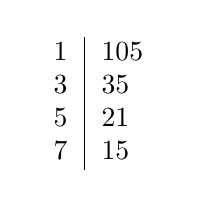
\begin{tikzpicture}
            \node at (0, 0) {
                \begin{tabular}{r|l}
                    1 & \fpeval{3*5*7} \\
                    3 & \fpeval{5*7} \\
                    5 &  \fpeval{3*7} \\
                    7 &  \fpeval{5*3}\\
                \end{tabular}
            };
        \end{tikzpicture}
    \end{center}
    
    \fpeval{3*5*7} a donc $8$ \textbf{diviseurs :} $1,3, 5, 7, 15,21,35,$ et \fpeval{3*5*7}.
    
\end{multicols}
}

%\columnbreak
\newpage

\boiteQFdet{Question 3 :}{

\textbf{Calcule} la somme des fractions suivantes : \[\dfrac{5}{18} + \dfrac{5}{2}\]

\tikz{\draw[dashed, line width=1pt] (0,0) -- (\linewidth,0);}

\vspace{-0.25cm}\begin{multicols}{2}

Pour \textbf{calculer} la somme des deux \textbf{fractions} $\dfrac{5}{18} + \dfrac{5}{2}$, nous devons d'abord les mettre sur un \textbf{dénominateur commun}.

Le \textbf{plus petit dénominateur commun} des dénominateurs $18$ et $2$ est $18$. Donc, nous convertissons chaque fraction pour avoir ce même dénominateur :


$\dfrac{5}{18}$ est déjà au dénominateur $18$

\columnbreak


\[
    \dfrac{5}{2} = \dfrac{5 \times 9}{2 \times 9} = \dfrac{45}{18}
\]

Ensuite, nous \textbf{additionnons} ces nouvelles fractions par leurs numérateurs :

\[
    \dfrac{5}{18} + \dfrac{5}{2} = \dfrac{5}{18} + \dfrac{45}{18} \\ = \dfrac{50}{18} = \dfrac{25}{9}
\]

Par conséquent,  $\dfrac{5}{18} + \dfrac{5}{2} = \dfrac{25}{9}$

\end{multicols}
}
%\end{multicols}